\chapter{Implementation}
-How implemented
\section{Approach}
\par The development approach taken focused on the business-logic, or back-end, of the system. From the two main possible development methodologies, Waterfall and Agile, the latter was used. In Waterfall, the devleopment process is a sequential process, where the dvelopment is considered as a sequence of phases that are completed one after the other (cite). In Agile, the focus in adaptive planning, evolutionary development, and continous improvement. The advantage of using an Agile approach over a Waterfall approach is that new features can be mplemented into the system easier. 
\par The most used way of using Agile methodology is through Sprint cycles. These are short development cycles, where a set of features must be implemented, alongside their tests to ensure the correctness of features(discussed in the Testing section). For this project, the cycles combined with the supervisor meetings. Since in them, the new features that were implemented were discussed alongside the new features that were to be implemented in the next cycle. 
\par A clear example of the advantage of this system was when the a new timeline view was suggested. In this new view, rather than having the events row by row, events that occurred during the same time period should be grouped. In addition, events that happened within that time period should be encapsulated by the larger events. This could be implemented in the system, due to the separation of the business logic and the view, and the development approach used. In a Waterfall model, the development is more structured, and thereby it is extremely useful for static requirements, i.e. requirements that will not change. However, in this case it would have caused issues in implementing the new view as it would require going up the Waterfall if the view of the system had already been implemented, or waiting until that step of the waterfall had been reached.
\par While the Agile methodology is mostly used in software development teams, it can be applied to single development projects. Since the structure allows for reviews of features which can be matched with supervisor meetings, and changes in the requirements of the project.
\section{Tools \& Software Libraries}
-development environment
-why used that environment
-software libraries (include an example use)
-why
\par The development environment of the project is a 64-bit Windows 10 machine, with a Intel Core i7-6700HQ CPU at 2.60GHz and 16.0GB of Random Access Memory (RAM). It includes a Java Intelligent Development Environment (IDE), with Git for version-control, and Gradle for dependency management. 
\par The use of verion-control allows development of features separata of working code, and only adding them to the working version if the required tests pass. It should be noted that Git flow was used. This involves having a develop branch with the newest working features of the system. The master branch will only contain the lastest fully implemented working version of the product. This allows for mistakes in development to be rolled-back to a state where the system worked correctly.
\par Gradle allows for libraries to be regarded as dependencies of the project. Such that when the system is ran on a separate machine, it will retrieve all the missing libaries used in the project before compiling and running the program. This allows for the system to be shared to other users, without having to include the libraries with the distribution of the code, as the required libraries and the version will be downloaded to the users system when they run the command: \makebox[\textwidth]{ \textbf{gradlew run}.} Where the gradlew is a wrapper for gradle, such that the user does not even have to have Gradle in their system to launch the system. This provides obvious advantages of portability and general use.
\par As mentioned in the Background chapter, multiple libraries exist to aid the task of Natural Language Processing. These are especially needed for the Named Entity Recognition(NER) and Text Summary task. As an NER annotator will tag certain words, or collection of words into predefined categories such as People, Companies, Locations, and Money. This is extremely useful for the task of identifying dates in sentences, and the subjects described in the sentences. In addition, these tools can aid in the tagging of words using the P.O.S Treebank, which is required for the implementation of the Hedge-Trimmer algorithm \cite{dorrzajicschwartz2003} for headline generation (i.e. summary of a sentence). The main advantage of using libraries for this task over developing these annotators, is that building such an annotator requires multiple developers and many years of work. This can be seen from the 	release history of the StanfordCoreNLP tool which intially released in 2010, but still in October 2016 new releases have been made\footnote{\url{http://stanfordnlp.github.io/CoreNLP/history.html}}. The main two NLP tools are Apache's OpenNLP\footnote{\url{https://opennlp.apache.org/}} and Stanford's CoreNLP\footnote{\url{http://stanfordnlp.github.io/CoreNLP/index.html}}. For this project the Stanford's tool was used in the implementation, as it provides an extended documentation and examples of using their tools, along with specific sections for each of their annotators. The Stanford tool is the main library used throughout the project, as the project is reliant on its NER and POS annotators (cite the stanford annotators). It comes with models, that are loaded during the initialisation of the system. These models are used in the annotators to determine whether certain words fall in predefined categories, or which POS tag should be given to them, through the use of statistics that are based on the models. 
\par As the two main NLP libraries available are Java implementations, the decision was made to build the system in that language. It would be problematic to build the system in a different language to its libraries, as it would require to make the two programming languages communicate with each other, which can cause unpredictable problems in the development and execution of the system.
\par Additional libraries in the development include JUnit for Unit testing. This allows for features of the system to be developed and for them to be tested for correctness. With the addition of the Git flow, when new features are developed, they are done on a separate branch. Before they are joined to the latest working version of the system the tests for other features and the current developed feature can be ran, thereby ensuring that the system is still working as expected even with the new feature. Unit testing allows for part of a system to be ran, and then to produce a result and compare it to an expected result. The test would then pass if the results match. Testing will be further discussed in one of the following sections.
\par Libraries for text extraction of .pdf and .docx file types are required, as the enconding of these files is not in a plain text model. Therefore the Apache POI\footnote{\url{https://poi.apache.org/}} and the Apache PDFBox\footnote{\url{https://pdfbox.apache.org/}} are used. In addition to text extraction, the PDFBox library along with the Apache Commons library allows the creation of PDFs (with text wrapping), which is required to save the timeline as a PDF. The Google GSON\footnote{\url{https://github.com/google/gson}} library is used for the creation of JSONs, which is required to produce an intermediate JSON of the timeline. The RichTextFX\footnote{\url{https://github.com/TomasMikula/RichTextFX}} library along with JavaFX are used to build the graphical interface of the system. All of the libraries included are provided with licenses that allow its use in systems, along as the system is made publicly available, which will be done as the resulting system will be open-source.

\section{Issues}
\par Two main issues arised during the implementation of the system. The creation of exact dates for named  entity dates and the creation of a encapsulated timeline. In addition, a minor issue in the system is input of documents that are grammatically incorrect.
\subsection{Named Entity Recognition (NER) of Dates}
\par The StanfordCoreNLP tool, allows the resolution of temporal expressions. To explain this, an example is presented. For example, the Stanford tool allows for reference dates be used when a document is processed. When the tool tags a temporal expression as DATE, it allows for this temporal expression to be normalized. The annotator treats each word in the sentence as a mention. To identify its named entity recognition tag, the following is done on the mention: 
\makebox[\textwidth]{\textbf{mention.get(CoreAnnotations.NamedEntityTagAnnotation.class)}.}
If it is a temporal expression that was tagged, the result of the operation is a String DATE (to identify it as a date). Thus, from the mention, it can be normalized using: \par
\makebox[\textwidth]{\textbf{mention.get(CoreAnnotations.NormalizedNamedEntityTagAnnotation.class)}.}
The Stanford tool will attempt to produce a date in the ISO 8601\footnote{\url{https://www.cl.cam.ac.uk/~mgk25/iso-time.html}} format. As can be seen from the format, it can produce exact dates of the type dd-MM-yyyy. Where dd is an integer value from 1 to 31, MM is the month as an integer value from 1 to 12, and yyyy the year. In addition, if BC dates are used, at the start of the normalized result a '-' is added. Using the ISO standard, a method was written to process these dates. However, in addition to the possible dates given by the ISO standard, Stanford builds on top of the standard, producing 3 additional Date normalizations.
\par The normalizations refer to temporal expressions that are ambigious even with a reference point. For example, the temporal expression "now" would produce a normalized NER: "PRESENT\textunderscore REF", i.e. a reference to the present moment. For a temporal expression that refers to the past, e.g. "...they once used to...", "once" would be normalized to "PAST\textunderscore REF", i.e. a reference to the past of this moment. For a temporal expression that refers to the future, e.g. "In the future..., "future" would be normalized to "FUTURE\textunderscore REF", i.e. a reference to the future after this moment. The issue with these normalizations is that the do not allow for the comparison of events used to sort them, as the start and end dates of events cannot be compared. To allow for comparison, the most possible general dates for these references are derived. Since a "PRESENT\textunderscore REF" refers to the present moment, it can be deducted that it represents the moment in which the text was written in, as that is the time context in which the author wrote it in. Thereby, the decision was made to produce as a general date for "PRESENT\textunderscore REF" the reference point provided by the user. Since the reference point is supposed to be the date in which the text was written in, it would be appropriate to link a reference of the present moment to it. The user can change the reference point to when-ever they would like not just the assumed date of the written document, but a present reference should match the base date used by the system to determine all other ambigious dates. For "PAST\textunderscore REF" and "FUTURE\textunderscore REF" a range of dates is used, i.e. a start and end date. For the former, the start date of the era is used, i.e. 01-01-0001, and a end date to the reference point. Since it can be determined that a ambigious mention of the past would fall anywhere within that time period, however an exact determination cannot be made as the temporal expression is not precise enough. For the latter, the start date is the present moment, i.e. the base date, and the end date is the last possible allowable date in the system, i.e. 31-12-9999. Since it would be appropriate for a mention of the future would refer to a moment from now (i.e. the present moment in which the text is presumed to be written in), up until the end of times. However as a limitation to our system, the end of times is considered the date 31-12-9999. This detection part of the normalized NER for Dates is presented as a snippet of the method that produces the exact dates from Normalized NER dates (see Figure \ref{fig:refCode}).
\par Even though the StanfordCoreNLP library is well documented, it was difficult to find all the template outputs of the tool when Normalizing NER Dates, as no file was initially found that pointed to all the outputs (specifically the "REF" outputs). However, afterwards it was found that the tool uses TimeML for the normalized dates, thus the templates could be found \footnote{\url{http://www.timeml.org/timeMLdocs/TimeML.xsd}}. 
\begin{figure}[H]
\begin{lstlisting}
private ArrayList<Date> getDate(String date) {
	...
	/* Set up variables for processing */
	if (onlyPastRefPattern.matcher(date).matches()) {
            //past so make range from 0001-01-01 -> base date (range)
            if (yearMonthDayPattern.matcher(baseDate).matches()) {
                //base date has the format yyyy-MM-dd
               /*split it and set the values in date1,month1, year1 of 
		the start year 01-01-0001*/
		/*and the end date values of date2, month2, year2 
		to the base date data*/
		...
            }
        } else if (onlyPresentRefPattern.matcher(date).matches()) {
            if (yearMonthDayPattern.matcher(baseDate).matches()) {
                //base date has the format yyyy-MM-dd
		/*set day1,month1,year1 to the data in the base
		 date data*/
		...
            }
        } else if (onlyFutureRefPattern.matcher(date).matches()) {
            if (yearMonthDayPattern.matcher(baseDate).matches()) {
		//set the day1,month1,year1 to the base date data
            }
           //set year2,month2,day2 to the end year 31-12-9999
        }
	...
	/* date1,date2,month1,month2,year1,year2 are 
	then used appropriately to generate dates used 
	for the event that holds this Timeline Date */
}
\end{lstlisting}
\caption{Part of the Implementation of Resolution of Normalized NER Dates}
\label{fig:refCode}
\end{figure}
\subsection{Encapsulated Timeline View}
\par The initial representation of the events was a traditional timeline (see Figure \ref{fig:traditionalView}). This view is effective when the events are on separate time periods, as it presents them one after the other in a sequence. However, when there are multiple events that occur during the same time period, they still appear one after the other. The issue is that unless the user specifically looks at the dates associated to the event, it will look at a first glance as events occuring in different time periods. This clearly violates the visibility objective of the user-interface of the system. A solution to this issue is to provide two views, the traditional timeline view which is effective at displaying events that have disjoint dates. The other view, is one where dates encapsulalte other dates, and hold the events that occur in that time period. For example, if there is more than one event that occurs on the "25-01-2017", then isntead of listing them both of these events are below the same date. This canthey cause a "bin-placing" problem. This where there are a set of bins, or in this case a set of graphical events, and they need to fit in a finite area(cite), in this case a box of certain width and height. However, this problem can be avoided through the use of scrollbars, which provides a container of infinite height, thereby all the bins (graphical representation of events) can be placed. This view has been called the "Range View". However, producing this view, requires placing the Results (the events of a set of documents) in Ranges (a data structure that can have one date, or a start and end date). The theory was discussed in the Design Chapter.
\begin{figure}[H]
\caption{Screenshot of the Traditional View of the Timeline of Events}
\label{fig:traditionalView}
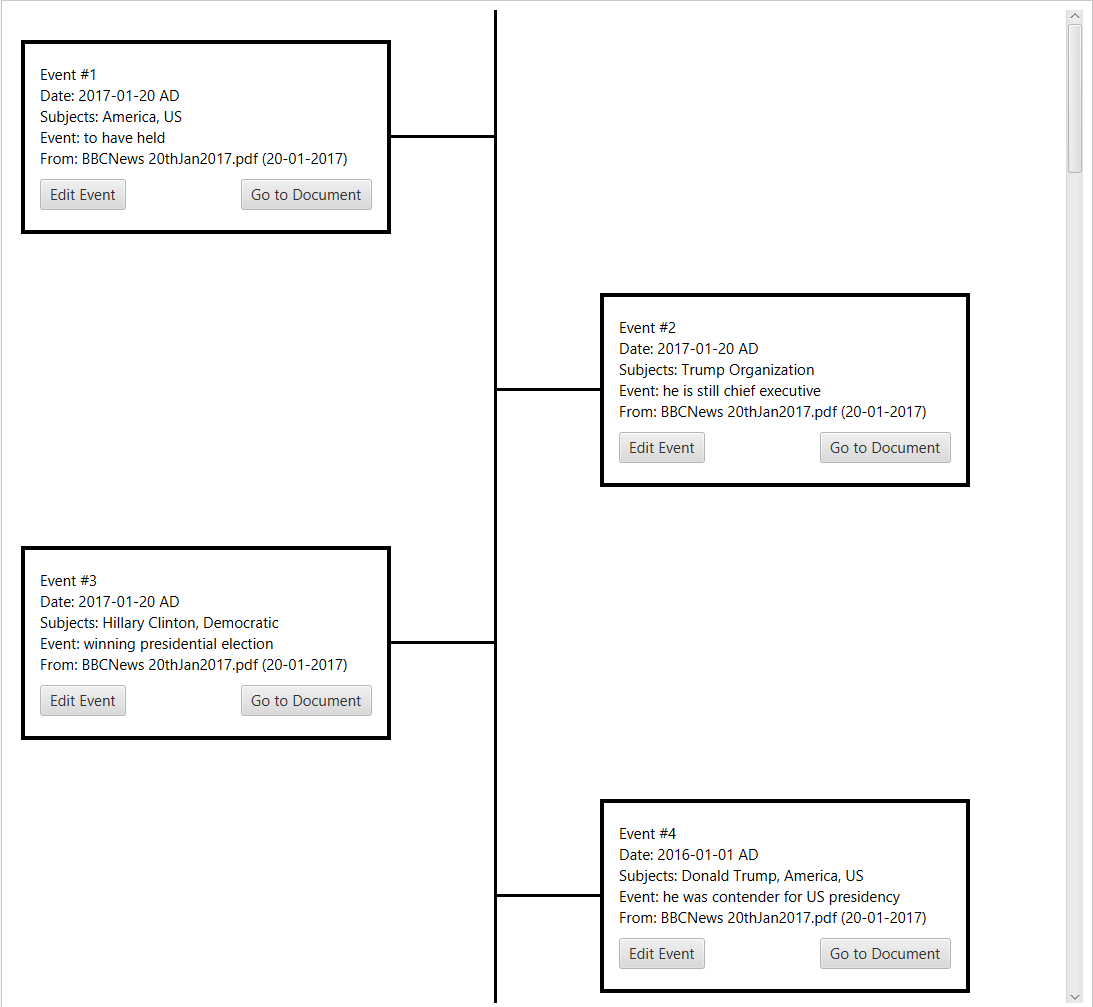
\includegraphics[width=\linewidth]{traditionalView.png}
\centering
\end{figure}
\par The theory behind the Range View, is having a list of Ranges, where each Range is a root node of a Tree of Ranges. Where each Range may hold zero or more Results (i.e. events), and a set of children Ranges (zero or more). When the timeline needs to be produced, the list of Roots is iterated over, assuming the list is of Roots has been sorted in the order of the start date, for each a GridPane is made. A GridPane is a layout which consists of rows and columns that can contain subviews (where a subview is a view, i.e. a graphical component). In the first column of the of the layout, the current Range's data is placed (i.e. the date(s) and the Results held), and in the second column the layouts of the child Ranges is recursively made. The algorithm is presented in Figure \ref{alg:rangeLayout}, it is done for each root Range in the list of Ranges to be created.
\begin{algorithm}[H]
\underline{function getRangeLayout(list l)}\;
\SetKwInOut{Input}{Input}
\SetKwInOut{Output}{Output}
\Input{A list of Ranges, of size $n$, to add in the first column}
\Output{a layout that encapsulates the Ranges passed in the input, and their child Ranges}
GridPane toReturn\;
toReturn set the number of rows to the size of the input\;
toReturn set the number of columns $:= 2$\;
\For{i $:=$ 0 $\shortrightarrow$ n}{
	Range $:=$ input list at $i$\;
	set up layout for this Range, and set it in toReturn at position $(i,0)$\;
	set its column span at $(i,0)$ to remaining\;
	get layout for the children of this Range $:=$ getRangeLayout(range.children)\;
	set this layout in toReturn at position $(i,1)$\;
}
return toReturn\;
\caption{Pseudo-Code of the Recursive Production of the Range Layout}
\label{alg:rangeLayout}
\end{algorithm}
\par The full implementation can be found in the Appendix. In the implementation, it was deceided to include 3 columns, to have a separator between a Range and its children Ranges, to improve the visibility of the system. Allowing the user to differentiate a Range and its child Ranges, and thereby differentiate the Results they hold. The individual layouts of Range is the listing of the Results in that Range (i.e. in the time period of that Range), and the date or start and end date for that Range. An example look of the Range View can be found in Figure \ref{fig:rangeView}.
\begin{figure}[H]
\caption{Screenshot of the Range View of the Timeline of Events}
\label{fig:rangeView}
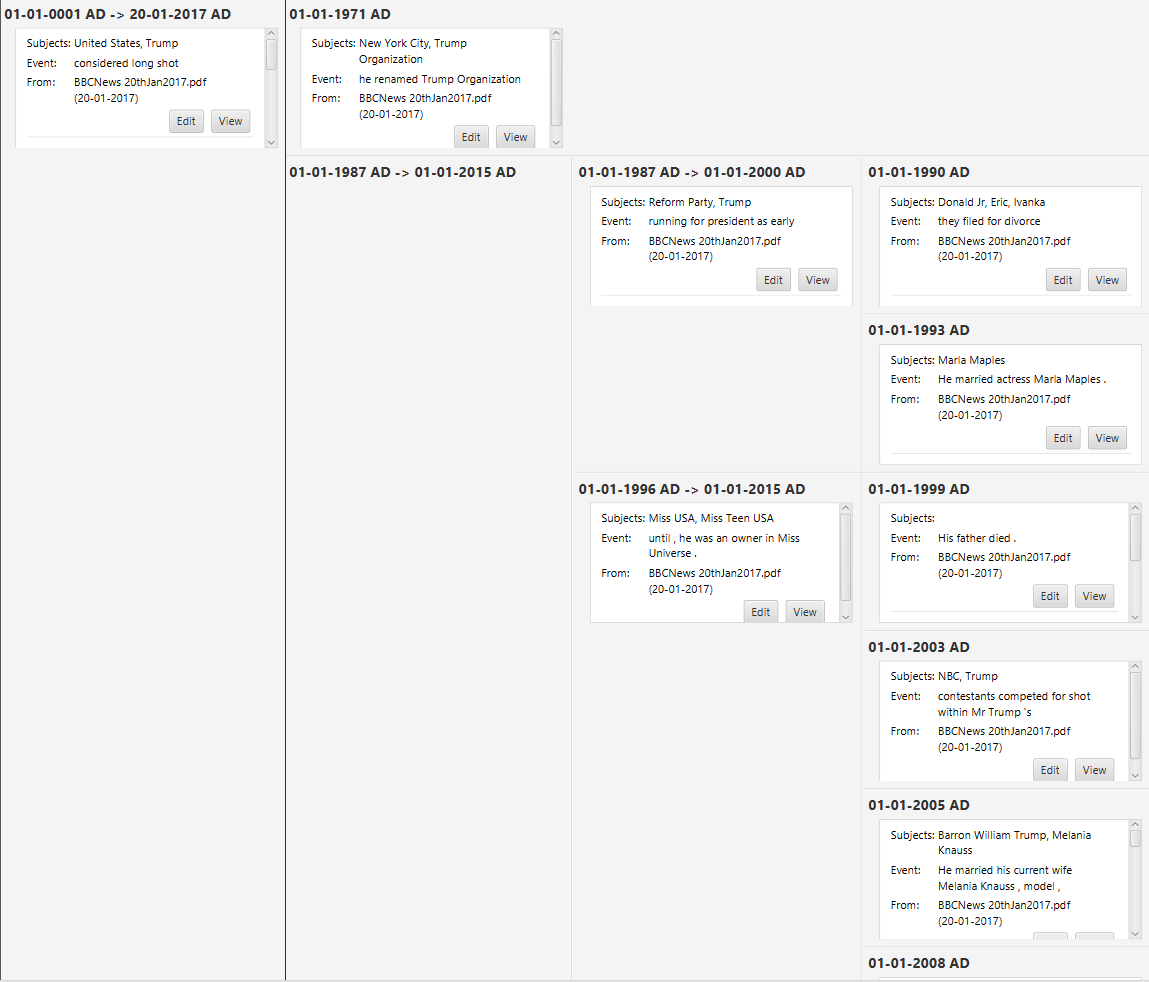
\includegraphics[width=\linewidth]{rangeView.png}
\centering
\end{figure}
\subsection{Incorrect Input Documents}
\par An important issue relating to the input documents is their format. NLP tools such as StanfordCoreNLP require a certain constraints to be assumed onto the input documents to be able to properly process them. Since these tools require assumptions to apply certain grammatical rules, it is extremely important that the documents are in correct English grammar. This was discussed in the Background Chapter along with a discussion of NLP tools being applied to Tweets, and how badly they performed. It is important that the documents are in English, as the models loaded by the StanfordCoreNLP in this implmentation are the English ones. All the other languages supported by the tool\footnote{\url{http://stanfordnlp.github.io/CoreNLP/human-languages.html}}, such as German, Spanish, and even Chinese require other models. The main implementation focus for the tool was the English language, but from when it was developed it was considered to be extended to other languages.
\par An issue that was discovered, was that separate sentences that a seperated by a period, but not a space following it, are treated as one sentence. The system still continues to work, however it can cause that only half of the events are detected, if every two sentences that have events are separated just by the period (and not the space). In addition, the summary would be applied to second sentence, as the rule of the algorithm details that the lowest-leftmost "S" subtree (i.e. sub-sentence) is picked. The start and end date of such an event, would therefore be the lowest date of the two events, and the highest date of the two events, due to how the dates of events are encapsulated in a TimelineDate object (that parses Normalized NER Dates, and updates the start and end dates it holds if a new min or max is found).
\par This issue can not be prevented, as it would require manipulation of the input documents, and it can be very likely the case that the user does not want the system to manipulate the input but rather just process it. Hence, it will be advised to users to ensure the documents are in English and grammatically correct. As the system will be used by law professionals, that are handling law documents, it can be assumed that these documents would follow this format, as law documents tend to be very formal texts.
-ner dates (explain, then present how to solve it through examples of code)
-new timeline view (present how to solve it through examples of code)
-minor issue of incorrect text
\section{Testing}
\par The focus of the testing in the system were Unit Tests. A Unit Test is when individual units (or pars) of source code of a system are tested to determine whether they are working correctly (cite). As the system was implemented in Java, the library used to aid this is JUnit\footnote{\url{http://junit.org/junit4/}}. Unit tests are primarily done on the back-end, or logic, of a system, as they focus on these parts to work correctly, and not the interaction of a user with the system. To test a users interaction with a system, Instrumentation tests are carried out. These involves emulating the users interaction with the system. Both the Unit and Instrumentation tests can be automated, such that they are carried out one after the other without the involvement of the developer.
\par The reason as to why only Unit Tests were used, is that the systems primary focus is its processing of documents, and not the graphical representation. The representation is used to display the results, however as disussed previously, the system could also just be used to process the texts, and the intermediate JSON used for a third-party visual representation. Hence, Instrumentation tests were not carried out.
\par A total of 35 tests were developed. The main advantage of these is that when new features are developed, to ensure that the system is still functioning correctly, the tests can be ran. If the test cases are appropriate, then it can be assured that the system will work correctly with the new features. This is aided additionally through the use of Git, where the features are developed on a separate branch of the current working version of code, and are only merged into the working version if all the test cases pass.
\par The tests focus was on the Engine (the component that takes as input text and produces lists of Results), the processing of Files (test files were used in this case), the production of Ranges, the changing of the systems states throughout the processing task, the parsing of Normalized NER dates, and the production of JSON's from a list of Results. Tests worked through assertions. Assertions are made where the expected output must match the actual output.
\par The tests were divided into three categories, a simple test, an intermediate test, and a complex test where all possibilities of input are tested. For example, for the production of Ranges, the complex test case expects multiple Range trees of different heights to be produced. The tests can be found in the Appendix. Due to the benefit of Gradle, the tests can be ran using the command:\par
\makebox[\textwidth]{\textbf{gradlew test}}
or, in the case the libraries need to be loaded:\par
\makebox[\textwidth]{\textbf{gradlew build}.}
In the build command, Gradle will not only run the test cases, but also produce the executable JAR which can be used to distribute the system as an executable to its non-developer users.
\section{UI}
//implementation ofthe UI.
\par From the wireframes presented in the Design Chapter, the actual User Interfaces (UI) were developed. The screenshots of the different windows are presented in the Figures below (see Figures \ref{fig:startUpImplemented}, \ref{fig:traditionalView}, \ref{fig:rangeView}, \ref{fig:editDialogImplemented}, and \ref{fig:viewDocImplemented}). As can be noted, the interface provides the requested functionality through the buttons and menus, but are missing color. Since the focus was on the processing of the text, a color palette was not developed for the system as it is believed that the system will be used for work related tasks, thereby its focus is not on enjoyment but rather functionality, visibility and simplicity. These objectives were attempted to be reached with this UI implementation.
\begin{figure}[h]
\caption{Screenshot of the Start Up View}
\label{fig:startUpImplemented}
\includegraphics[width=\linewidth]{startUpImplemented.png}
\centering
\end{figure}
\begin{figure}[h]
\caption{Screenshot of the Edit Dialog View}
\label{fig:editDialogImplemented}
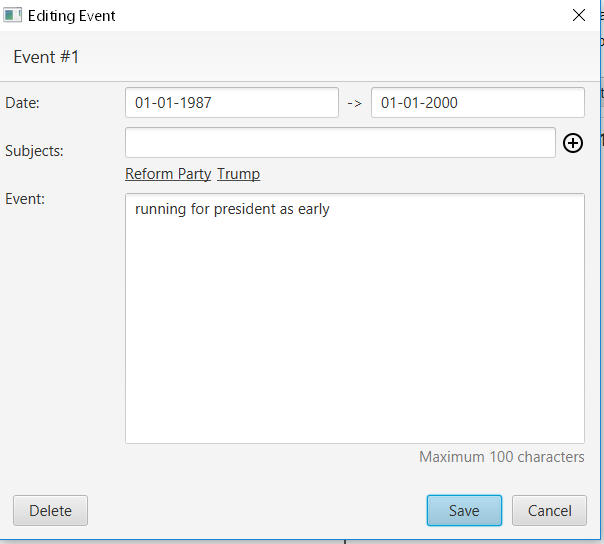
\includegraphics[width=\linewidth]{editDialogImplemented.png}
\centering
\end{figure}
\begin{figure}[h]
\caption{Screenshot of the Document Viewer}
\label{fig:viewDocImplemented}
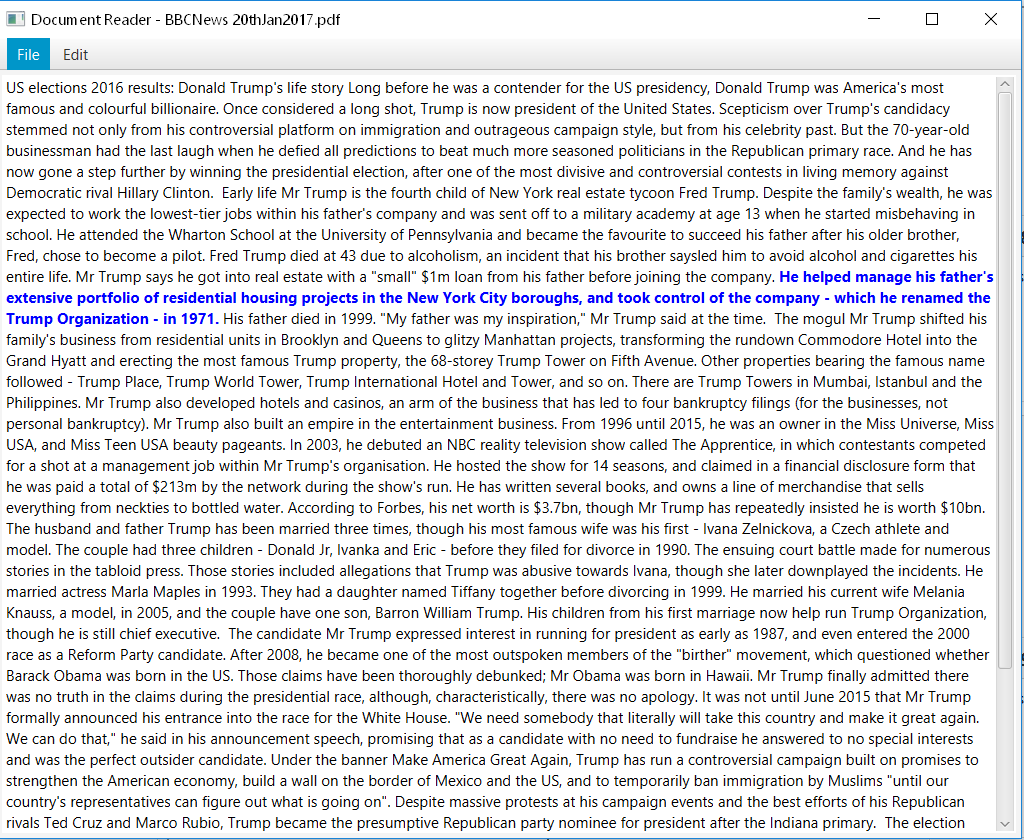
\includegraphics[width=\linewidth]{viewDocImplemented.png}
\centering
\end{figure}
\par It should be noted that in the Range view (see Figure \ref{fig:rangeView}) is zoomable. This allows the user to have a broader image of the Range View, if it is required. It may allow the user to obtain a general picture of what occurred.
\par The data presented of events includes the subjects and its summary. Since the events are encapsulated in Ranges, it is sufficient to show the date(s) for this Range at the top. Thereby intuitively demonstrating to the user that the following events occurred during that time period. This separates meta data from the event, e.g. when the event occurred, from the actual data which is what occurred in the event and what are the subjects of interests of the event. In addition, each event is accompanied by two buttons, which are both the relevant main operations: to edit the event (which includes deleting it, as can be seen from Figure \ref{fig:editDialogImplemented}, and to view the document that produced it.
\par An advantage of the Traditional View over the Range view, is memory efficiency. As the Range view has the function of being zoomable, i.e. the user can zoom in/out, due to language specific constraints, it cannot be implemented through a ListView. A ListView being a layout data structure where objects of a list are placed row by row. To avoid stack overflows if the list is to large, the ListView will only produce the graphical layout for the rows when they are needed (i.e. they need to be shown), and otherwise delete them. For example, for a list of 10000 items, it is very expensive to hold in memory the individual layouts of 10000 rows, even when only 5 are being shown. Instead only the 5 that are being shown are held in memory, and the rest are generated as necessary. This is not the case with the Range View, as a tradeoff was made to allow the zoom function. As the memory capicity of personal computing systems (where the tool is intended to be used, but is not limited to) is large, this would not be an issue for the processing of tens or hundreds of events, however for larger sets this would cause memory issues. Thus the traditional view is suggested in such case.
\section{Important Algorithms}
//highlight algorithm implementation: processing of files through semaphores, adding to ranges, pdf save and json save
\par This sections intended use is to present noteworthy algorithms. In specific their implementation.
\subsection{Processing Files}
\par The pseudo-code of the processing files was presented in the Design Chapter. It was also mentioned the use of semaphores, where they enforce that only $n$ processes can acquire their lock, with the $n+1$ process having to wait until a process releases its lock. However, the implementation is not trivial (see the Appendix). The system must allow a certain maximum number of threads to be ran in parallel to process documents. It must not fall in deadlock and starvation, that is when processes are waiting indefinetely to run, and thereby the system does not move ahead. Thus can occur when semaphores are used, and they are not released when a process finishes its task, in this case processing a file and producing a list of Results. Thus a callback is used when the Threads are used, this callback is to be used when the Thread finished it task. It will ensure that the semaphores are released. The processing of documents ensures that when an error occurs, a result is still produced, thus the thread should not finish and not use the callback. However, necessary multi-threading precautions must be considered. When the callback is used, data is also transferred (specifically the Results of processing the document) which can cause concurrency issues when two threads attempt to add to the result list at the same time. Fortunetely, Java provides the \textbf{synchronized} keyword for methods (see Figure \ref{fig:callbackFilesImplemented}). This ensures that no two threads may run the method at the same time. One thread must finish its execution of the method before another one can begin its execution. Thus dealing with the issue of adding to a list at the same time. 
%%Processing File was here
\begin{figure}[H]
\begin{lstlisting}
public synchronized void callBack(ArrayList<Result> results, FileData fileData) {
    //we finished processing a file
    filesToGo--;//one less to look at
    //add the results to the list held
    this.results.addAll(results);
    //release semaphore
    semaphore.release();
    //check if we have processed everything, 
    //if so release the finished semaphore
    if (filesToGo == 0) {
        //has processed
        BackEndSystem.getInstance().setSystemState(SystemState.PROCESSED);
        //has returned the results so we finished
        BackEndSystem.getInstance().setSystemState(SystemState.FINISHED);
        semaphoreFinished.release();
	    //value is now 1, so the thread that was acquiring can continue
    }
}
\end{lstlisting}
\caption{Implementation of Callback after Files have been processed}
\label{fig:callbackFilesImplemented}
\end{figure}
\par Threading precautions have been taken throughout the project. Where threads and data are used, it is ensured that the data can be processed independently of itself to allow for parallelism. Where this is not the case, synchronization and semaphores are used to ensure that concurrency issues are dealt with.
\subsection{Building Ranges}
\par The algorithm for building Ranges out of Results was presented in the Design Chapter. However, it was not described how it can is checked whether or not a Result can be added to an existing Range. When a Result is attempted to be added to a pre-existing Range, a \textbf{add()} (see Figure \ref{fig:addRangeImplementation}) method is called. In this method, it is initally checked whether the Result should be attempted to be added to this Range. This check involves looking at the dates of the Result and checking whether they are fully or partially encapsulated by the Range's dates. If this is not the case, then the attempt of adding the Result fails, otherwise the algorithm continues. Next it will be checked whether it can be added to any of the nodes of the Range tree, if there is any node that holds the exact same date(s) as the Result, i.e. the Result should be held by this Range. If this is the case then the Result will be added and that node, however if this is not the case, then it can be determined that the Result belongs to this Range, however its position in the tree needs to be created or a Range that partially encapsulates it needs to be expanded. This involves traversing the tree and finding the position where the new Range note should be placed, or expanding a Range and moving subtrees to maintain the structure of the Range tree.
\begin{figure}[H]
\begin{lstlisting}
public boolean add(Result result) {
    TimelineDate timelineDate = result.getTimelineDate();
    //check constraints
    if (!shouldAdd(timelineDate)) {
	//check constraints if we can even add to this range
        return false;
    }
    //attempt to add through an existing range
    Range toAdd = checkCanAdd(result);
    if (toAdd != null) {
	//add to the results of the given range
        toAdd.results.add(result);
        return true;
    }
    //now we try to extend the range
    return createRangeAndAdd(result);
}
\end{lstlisting}
\caption{Implementation of Adding Results to a Range}
\label{fig:addRangeImplementation}
\end{figure}
\subsection{Saving Results}
\par Saving the results of the processed documents, is divided into two parts: saving them as a PDF, or as a JSON. 
\par In the PDF system, the file that is saved, is a graphical representation of the events, using the traditional timeline view. It is aided through the use of the Apache PDFBox and Commons library. The libraries work like a painting tool. The pages are canvises, where lines and text can be drawn on at specific positions. These positions are given by coordinates $(x,y)$, where the top left of the page is the origin, i.e. (0,0), and the x values increment towards the right of the page, and the y values towards the bottom of the page. To build a dynamic system, that can create a pdf for any number of Results, it requires certain constraints. Such as the maximum number of events to be displayed on each page, and the size of the text of the summaries and subjects. Due to issues with the tool, it is not possible to continue on the next page of the PDF, hence it is limited to how many events are shown and the size of the text (as it can overflow to the next page). However, since the text that is used in the summary, should  be short (since it is a summary), the constraint can be applied. Therefore, it can be assumed that there is a max size of the container that holds one event. This allows for every container to be of this max size, to avoid the issue of resizing containers depending on the amount of text. Therefore, the system can be considered as drawing containers on the page and filling them with the data, moving along to the next position and repeat. Hence the task, in the implementation, has been broken down to padding, writting text, and drawing the rectangle. Since in the traditional view, the layout of the events are one on the left and the next on the right, the tasks have to be changed minimally to allow for this. The full implementation can be found in the Appendix. As an example, the Figure \ref{fig:drawRecImplemented} has been provided to demonstrate the task of drawing for an event that is to be placed on the right of the page.
\begin{figure}[H]
\begin{lstlisting}
private void drawOddEvent(Result result, PDPageContentStream contentStream, int position) throws IOException {
	//initially y is the top right where this needs to 
	//be shown, x starts from the middle
	currentY -= padding; //add some padding to y
	currentX = (int) widthOfPage / 2;
	contentStream.moveTo(currentX, currentY);
	//write the text for the Event
	int lengthOfHorLine = (int) ((widthOfPage / 2) - (padding + widthOfRectangle));
	currentX += lengthOfHorLine;
	writeText(result, contentStream, currentX, position);
	//draw the rectangle to surround the text
	drawRectangle(contentStream, currentX, currentY - heightOfRectangle);
	//draw the horizontal line connecting event timeline
	currentY -= heightOfRectangle / 2;
	contentStream.moveTo(currentX, currentY);
	contentStream.lineTo(widthOfPage / 2, currentY);
	contentStream.stroke();
	currentY -= (heightOfRectangle / 2) + padding;
}
\end{lstlisting}
\caption{Implementation of drawing for a Result in the PDF timeline}
\label{fig:drawRecImplemented}
\end{figure}
\par In the JSON implementation, it is aided by the use of the Google GSON library. The advantage of this library is that it allows for a flexible creation of JSONs. In specific, it allows the developer to specify how an object of a given type should  be serialized (see Figure \ref{fig:adapterGsonImplemented}). In this implementation, the objects to be serialized are Result objects. The data to be added for them is the dates, the subjects, the summary and the relevant data of the file that produced it. This can be done through defining the adapter to be used for the objects of the Result class. In the adpater the resulting \textbf{JsonObject} can be created, the data can be set in it, and then return it. For a list of Results, this will be carried out for each Result, and thereby a resulting list of JsonObjects will be returned, i.e. a JsonArray. This can then be saved by the user in a file, and can be interpreted by ay third-party system, as this is the use of JSON and the format of each event (Result) is clearly defined with key-value pairs. The format of a JSON of a Result is given in Figure \ref{fig:jsonResult}. Where G in the dates is the ERA (i.e. BC or AD) of the date.
\begin{figure}[h]
\begin{lstlisting}
{
"date1":dd-MM-yyyy G,
"date2":dd-MM-yyyy G,
"subjects":[],
"event":String,
"from":{
	"filename":String,
	"baseDate":dd-MM-yyyy
	}
}
\end{lstlisting}
\caption{Structure of Result (event) JSON}
\label{fig:jsonResult}
\end{figure}
\begin{figure}[H]
\begin{lstlisting}
public JsonElement serialize(Result src, Type typeOfSrc, JsonSerializationContext context) {
	//json object for this result
    	JsonObject jsonObject = new JsonObject();
	//adding the range dates (which can be null)
	/* whenever a value is null, the key-pair will not be included in the final JSON */
	jsonObject.addProperty("date1", src.getTimelineDate().getDate1FormattedDayMonthYear());
	jsonObject.addProperty("date2", src.getTimelineDate().getDate2FormattedDayMonthYear());
	//adding the subjects
	JsonArray subjectJsonArray = new JsonArray();
	for (String subject : src.getSubjects()) {
		subjectJsonArray.add(subject);
	}
	jsonObject.add("subjects", subjectJsonArray);
	//adding the event
	jsonObject.addProperty("event", src.getEvent());
	/*adding the file data (excluding the path, since this can be used on other system where files are elsewhere)*/
	JsonObject fromJsonObject = new JsonObject();
	FileData fileData = src.getFileData();
	if (fileData != null) {
		fromJsonObject.addProperty("filename", fileData.getFileName());
		fromJsonObject.addProperty("baseDate", fileData.getCreationDateFormattedDayMonthYear());
	}
	jsonObject.add("from", fromJsonObject);
	return jsonObject;
}
\end{lstlisting}
\caption{Implementation of the Serializer used in the Adapter to generate JSON for a list of Results}
\label{fig:adapterGsonImplemented}
\end{figure}

-main algorithms: for building events, building ranges, pdf save, json save, processing files
